\documentclass[journal]{IEEEtran}
\usepackage[T1]{fontenc}
\usepackage{amsmath,amssymb}
\usepackage{graphicx}
\usepackage{url}
\usepackage{booktabs}
\usepackage{array}
\usepackage[hidelinks]{hyperref}
\graphicspath{{fig/}}
\makeatletter\g@addto@macro{\UrlBreaks}{\do\_\do\-\do\.}\makeatother
\DeclareUrlCommand\repo{\urlstyle{tt}}
\newcommand{\gene}[1]{\textit{#1}}
\newcommand{\twofig}[2]{\includegraphics[width=0.49\columnwidth]{#1}\hfill\includegraphics[width=0.49\columnwidth]{#2}}
\markboth{Preprint}{Preprint}

\begin{document}

\title{Gene Regulatory Network Construction in Fragile X Syndrome:\\
An Integrative Transcriptomic, Epigenomic, and Permutation-Tested Computational Framework Across Two Independent Cohorts}

\author{Aditya~Jha and Softya~Sebastian%
\thanks{A.~Jha and S.~Sebastian are with Vellore Institute of Technology, Chennai, India (e-mail: aditya.jha@vitstudent.ac.in; softya.sebastian@vit.ac.in).}%
\thanks{All code, intermediate results, result tables and figures are available at \url{https://github.com/adj-04/fxs-research}. Supplementary tables and figures referenced as S1--S12 are files in that repository (Table~\ref{tab:supp}).}}

\maketitle

\begin{abstract}
Fragile X syndrome (FXS) arises from CGG-repeat expansion and promoter hypermethylation at \gene{FMR1}, but how this single silencing event reorganizes the broader transcription-factor (TF) regulatory landscape is poorly characterized. We built a multi-omics pipeline combining bulk RNA-seq differential expression (DESeq2), Illumina 450K methylation analysis (limma), and GENIE3, PANDA, LIONESS and ALPACA network inference, applied to two independent NCBI-reprocessed RNA-seq cohorts (iPSC-derived cerebral organoids, $n=12$; NPC/B-lymphocyte/iPSC, $n=10$) and one peripheral-blood methylation cohort ($n=62$). \gene{FMR1} silencing replicated across all three datasets (log$_2$FC $-10.47$ and $-8.91$; mean $\Delta\beta=0.56$ across 15 probes). Beyond \gene{FMR1}, cross-cohort concordance was weak (genome-wide sign concordance 50.6\%, Pearson $r=0.034$), and permutation nulls showed that no GENIE3 edge, PANDA edge or ALPACA node survived FDR $<0.05$. A tissue-generality classification across the three tissue contexts found \gene{FMR1} to be the only gene significant in more than one, indicating that most downstream change is tissue-restricted. In silico validation nonetheless recovered previously reported FXS-associated regulators: SP1 (TRRUST enrichment, FDR $=3.5\times10^{-6}$) and REST/NRF1 (rank 1 of 200 by ENCODE self-recovery) were locally central within their regulatory modules, although none ranked among genome-wide hubs. We report negative and marginal results alongside positive ones, and argue that at the sample sizes available for a rare monogenic disorder, network-level regulatory inference is best treated as hypothesis-generating. All code, intermediate results and figures are publicly released.
\end{abstract}

\begin{IEEEkeywords}
Fragile X syndrome, gene regulatory network, GENIE3, PANDA, LIONESS, ALPACA, DNA methylation, permutation testing, cross-cohort validation, tissue specificity.
\end{IEEEkeywords}

\section{Introduction}
\IEEEPARstart{F}{ragile} X syndrome (FXS) is the most common inherited cause of intellectual disability and a leading monogenic contributor to autism spectrum disorder~\cite{santoro2012}. It results from expansion of a CGG trinucleotide repeat in the 5$'$ untranslated region of \gene{FMR1}~\cite{peprah2012}, which triggers promoter hypermethylation, transcriptional silencing, and loss of the fragile X messenger ribonucleoprotein (FMRP)---a process linked to broader genome instability at repeat-expansion loci~\cite{hayward2021}. FMRP normally regulates translation and localization of a large set of neuronal mRNAs, so its loss has knock-on effects across synaptic development, neuronal maturation, and cognition.

Prior transcriptomic and epigenetic work has mapped the downstream expression changes tied to \gene{FMR1} silencing in reasonable depth~\cite{li2020,malachowski2023}, and reversing promoter methylation has been shown to partially restore neuronal phenotypes in patient-derived models~\cite{liu2018,brykczynska2016}. What has received comparatively little attention is how the TF regulatory architecture itself is reorganized once \gene{FMR1} is lost, and---just as importantly---whether that reorganization is something small FXS cohorts can actually detect with statistical confidence.

We state our contribution precisely up front to avoid any ambiguity: the CGG-repeat $\rightarrow$ promoter-hypermethylation $\rightarrow$ \gene{FMR1}-silencing mechanism is already well established~\cite{peprah2012,hayward2021,liu2018,brykczynska2016}, and this paper does not claim to revise it. \gene{FMR1} silencing is reproduced here purely as an internal validity check---proof that the sample labels, processing pipeline, and cohorts behave as expected---not as a novel finding. The contribution this paper makes is downstream of that mechanism, and has two parts: (i) a permutation-tested, cross-cohort-validated framework for asking whether network-level regulatory reorganization following \gene{FMR1} loss is statistically detectable at realistic FXS sample sizes, and (ii) an explicit classification of which downstream transcriptional and methylation changes are shared across tissue contexts versus specific to one, using the three independently derived tissue sources available here (cerebral organoid, NPC/B-lymphocyte/iPSC, and peripheral blood) as three deliberate probes rather than as a confound to be averaged away. We report both parts honestly, including where they come back negative or inconclusive.

Standard differential expression analysis tells you which genes change on average between cases and controls, but it does not directly model how the regulatory interactions between genes shift. Gene regulatory network (GRN) inference addresses this by modeling TF--target relationships explicitly, which can in principle surface regulatory rewiring even among genes whose average expression barely moves. GENIE3~\cite{genie3} infers TF--target interactions from expression data using tree-based ensemble regression; PANDA~\cite{panda} combines expression with TF motif and protein--protein interaction (PPI) priors through iterative message passing; LIONESS~\cite{lioness} extends PANDA to estimate sample-specific networks; and ALPACA~\cite{alpaca} identifies differential community structure between two network conditions.

This work assembles those four methods into a single pipeline and applies it to FXS, with two additions we think matter for a disorder this rare: (i) validation against a second, independently processed RNA-seq cohort rather than a single dataset, and (ii) permutation-based null models for every network-level statistic we report, so that apparent structure can be distinguished from what tree-based and message-passing methods produce on this few samples by construction. Both additions changed our conclusions substantially relative to a single-cohort, no-null-model version of this pipeline, which is part of why we think they are worth reporting alongside the positive findings.

Concretely, the pipeline (Fig.~\ref{fig:workflow}):
\begin{enumerate}
\item runs differential expression on two independent bulk RNA-seq cohorts using DESeq2;
\item runs differential methylation analysis on an independent 450K methylation cohort using limma;
\item infers baseline TF--target interactions with GENIE3, restricted to a curated TF list and the transcriptome, and quantifies how much of the transcriptome that restriction leaves eligible as a target in the first place;
\item builds a PANDA network from JASPAR motif priors, STRING PPI priors, and a continuous methylation-derived promoter-accessibility weight;
\item estimates sample-specific networks with LIONESS and bootstrap-tests whether FXS networks are systematically stronger than control networks;
\item identifies differential modules with ALPACA and tests their significance against a permuted null;
\item classifies genes as tissue-general or tissue-specific across the three available tissue contexts;
\item validates candidate regulators in silico against ENCODE ChIP-seq and TRRUST; and
\item cross-validates DEGs and effect sizes between the two RNA-seq cohorts using rank--rank hypergeometric overlap (RRHO) and genome-wide effect-size correlation.
\end{enumerate}

We see this less as a claim of a fully resolved FXS regulatory network and more as a template for what a rigorously validated---and honestly reported---computational framework looks like when the underlying patient data is, as it almost always is for a rare monogenic disorder, too small to power network inference on its own.

\section{Related Work}
Malachowski et al.~\cite{malachowski2023} used spatial heterochromatin mapping to show coordinated silencing of long synaptic genes in FXS, producing one of the more comprehensive transcriptomic resources currently available; a matched cohort processed by NCBI from that study's raw data forms our validation dataset. Li et al.~\cite{li2020} built molecular interaction networks around FMRP-regulated transcripts using graph diffusion, but focused on RNA-binding targets rather than TF-mediated regulation. Patient-derived pluripotent stem cell studies~\cite{boland2017,lu2016} and mouse-model studies~\cite{rogers2017,arsenault2021} have each characterized pieces of the transcriptional and neurodevelopmental phenotype, and epigenetic editing studies~\cite{liu2018,brykczynska2016} have established promoter methylation as central to \gene{FMR1} silencing. Broader systems-biology work on network-based disease-gene prioritization~\cite{nitsch2009} and FXS mouse-brain metabolomics~\cite{davidovic2011} motivate the network-centric approach taken here.

On the methods side, GENIE3~\cite{genie3}, PANDA~\cite{panda}, LIONESS~\cite{lioness}, and ALPACA~\cite{alpaca} are each well established individually, and have been combined pairwise in various disease contexts. To our knowledge this is among the first frameworks to combine all four with (a) two independent RNA-seq cohorts, (b) permutation nulls for every network statistic, and (c) in silico ChIP-seq/TRRUST validation, specifically for FXS.

\section{Datasets}
Table~\ref{tab:datasets} summarizes the three public datasets used, all retrieved from NCBI GEO. Both RNA-seq cohorts use NCBI-reprocessed, gene-level counts (GRCh38.p13, Entrez gene IDs) rather than submitter-supplied quantifications, so differences between them cannot be attributed to quantification-pipeline artifacts. Sample metadata as used in the analysis are provided in the repository (\repo{data/GSE218676_metadata.csv}, \repo{data/GSE41273_metadata.csv}).

\begin{table*}[!t]
\centering
\caption{Datasets used in this study.}
\label{tab:datasets}
\begin{tabular}{@{}lllll@{}}
\toprule
Role & Accession & Modality & Design & Samples\\
\midrule
Primary & GSE146339 & iPSC-derived cerebral organoids (day 28, day 105) & FXS vs.\ Control, $\sim$ timepoint + condition & 12 (6 FXS, 6 Ctrl)\\
Validation & GSE218676 & Patient NPC / B-lymphocyte / iPSC & FXS vs.\ Control, $\sim$ cell type + condition & 10 (5 FXS, 5 Ctrl)\\
Methylation & GSE41273 & Illumina 450K methylation array, peripheral blood & FXS vs.\ Control & 62 (9 FXS, 53 Ctrl)\\
\bottomrule
\end{tabular}
\end{table*}

\begin{figure*}[!t]
\centering
\includegraphics[width=0.82\textwidth]{workflow_diagram.png}
\caption{Computational workflow for the proposed FXS regulatory network analysis. Each box is one stage of the pipeline; the flow runs left to right and wraps top to bottom.}
\label{fig:workflow}
\end{figure*}

The two RNA-seq cohorts differ in tissue and cell-type composition (cerebral organoid vs.\ NPC/B-lymphocyte/iPSC), and the methylation cohort adds a third, non-overlapping tissue context (peripheral blood). Rather than treating this as a nuisance to be adjusted away, we use it deliberately as three independent windows onto the same underlying lesion: a gene or region that shows a concordant effect in two or more of these tissue contexts is more plausibly a tissue-general consequence of \gene{FMR1} loss, while one that appears in only a single context is more plausibly tissue-specific rather than a false positive. This framing is only as strong as the assumption that discordance reflects biology rather than technical noise between processing pipelines; we mitigate this specific concern by using NCBI-reprocessed, gene-level counts for both RNA-seq cohorts. The methylation cohort remains a population-level, non-matched third tissue---it does not have paired RNA-seq from the same individuals---so its role is limited to indicating whether promoter-level epigenetic changes are similarly tissue-general or focal, not to matched multi-omic integration.

\section{Methodology}
\subsection{Workflow Overview}
Figure~\ref{fig:workflow} summarizes the overall pipeline. RNA-seq (both cohorts) and methylation data are processed independently before being harmonized against a curated TF list. GENIE3 and PANDA build baseline regulatory networks; LIONESS extends PANDA into sample-specific networks; ALPACA identifies differential modules between FXS and control aggregate networks; and every network-level result is re-evaluated against a permutation-derived null before being interpreted biologically. In silico validation and cross-cohort concordance testing close the loop. The full pipeline is implemented as three sequential R scripts (\repo{scripts/part1_steps1-8.R}, \repo{scripts/part2_steps9-16.R}, \repo{scripts/part3_steps17-19.R}).

\subsection{RNA-seq Differential Expression}
Gene-level counts for both cohorts were obtained as NCBI-reprocessed GRCh38.p13 matrices and loaded alongside metadata-driven sample annotation. Counts went into DESeq2~\cite{deseq2}, with variance-stabilizing transformation applied for downstream network inference and the Wald test used for differential expression, at an adjusted $p$-value $<0.05$ and $|\log_2\mathrm{FC}|>1$. As a sanity check on sample labeling, we required \gene{FMR1} to be significantly downregulated in FXS before proceeding past this step in either cohort; both cohorts passed this gate cleanly. Full and significant result tables are given in Supplementary Tables S1--S2 (Table~\ref{tab:supp}).

\subsection{Differential DNA Methylation}
We processed beta-value methylation data from the Illumina HumanMethylation450 platform (GSE41273; 62 samples) using limma's empirical-Bayes moderated $t$-test framework~\cite{limma}. Probes were called significant differentially methylated positions (DMPs) at adjusted $p$-value $<0.05$ and $|\Delta\beta|>0.1$, with annotations drawn from the IlluminaHumanMethylation450k package via minfi~\cite{minfi}. Multi-gene probes were expanded, then aggregated to gene-level mean differences and classed as hyper- or hypomethylated by sign (Supplementary Table S3).

\subsection{TF List, Harmonization, and Target Eligibility}
A curated list of 1,390 known human TFs (\repo{data/tf_list.txt}) was intersected with the processed expression matrices; Ensembl/Entrez identifiers were mapped to HGNC symbols via \texttt{org.Hs.eg.db}, with unresolved symbols handled through batched Ensembl BioMart queries. After harmonization, 1,340 genes were retained for GENIE3 network construction. We flag explicitly that this leaves only 4.67\% of the full 28,679-gene expression matrix eligible as a GENIE3 target at all (\repo{results/GENIE3/GENIE3_restriction_bias_summary.csv}), and that the primary DEG set (13 genes) contributes only a small fraction of those targets---the resulting network is, in practice, close to a TF--TF network rather than a genome-wide TF--target network, and each known TF's motif regulon is correspondingly under-sampled (Supplementary Table S4, \repo{results/methylation/TF_target_eligibility_bias.csv}, quantifies this per TF). Six TFs previously reported in the FXS literature---SP1, NRF1, REST, FOXG1, SIX3, and TFAP2A---were set aside a priori as biological reference regulators, used only to check the recovered networks after the fact.

\subsection{Baseline Network Inference: GENIE3}
GENIE3~\cite{genie3} was run over the harmonized 1,340-gene expression matrix (1,000 trees per target), fitting per-target regression-tree ensembles with TF expression as predictors and taking feature-importance scores as regulatory-strength proxies. Edges with zero importance were discarded.

\subsection{Motif- and PPI-Informed Network Construction: PANDA}
A TF motif prior was built by scanning promoter regions of GENIE3-eligible target genes (hg38) with JASPAR 2020 TF binding motifs~\cite{jaspar2020}, restricted to TFs surviving harmonization. A PPI prior came from high-confidence STRING v12.0 human interactions between TF pairs~\cite{string2023}; TFs absent from STRING received low-weight self-interactions to keep the network complete. Unlike an earlier binary hyper/hypomethylated weighting scheme---which we found modulated only 0.12\% of prior edges and was uninformative---the motif prior here is reweighted by a continuous function of control-group promoter methylation, $1.5-\beta_{\text{promoter}}$ (Fig.~\ref{fig:methweight}; per-gene values in \repo{results/methylation/promoter_methylation_by_gene.csv}), so that the prior encodes baseline promoter accessibility rather than the FXS contrast itself. PANDA~\cite{panda} then ran the standard message-passing update to convergence on the expression matrix, motif prior, and PPI prior.

\begin{figure}[!t]
\centering
\twofig{methylation_weight_distribution.png}{methylation_weighting_effect.png}
\caption{Continuous methylation-derived promoter-accessibility weight. Left: distribution of the weight $1.5-\beta_{\text{promoter}}$ applied to the PANDA motif prior. Right: effect of this weighting relative to the earlier binary hyper/hypomethylated scheme.}
\label{fig:methweight}
\end{figure}

\subsection{Sample-Specific Networks: LIONESS}
Sample-specific networks were estimated with LIONESS~\cite{lioness} running in PANDA mode, one network per RNA-seq sample. For every TF--target edge, we computed the proportion of samples in which the edge weight was higher in FXS than in the mean control network, and bootstrapped this statistic (1,000 resamples) to obtain a 95\% confidence interval, rather than relying on a point estimate alone given the small sample size.

\subsection{Differential Modularity: ALPACA}
Aggregate FXS and control networks were built by averaging the corresponding LIONESS sample-specific networks within each group. ALPACA~\cite{alpaca} then detected community structure in the control network and computed differential modularity scores for the FXS network against it, yielding a set of candidate differential modules. The final annotated module network was exported in XGMML format (\repo{networks/FXS_ALPACA_network.xgmml}) for visualization in Cytoscape~\cite{cytoscape}.

\subsection{Permutation Nulls}
For GENIE3, PANDA, and ALPACA, we additionally built null distributions by repeating the relevant inference step on label-permuted or randomized-prior data (20 PANDA permutations; label-shuffled nulls for GENIE3 and ALPACA), and re-expressed each nominally significant edge/node/module as an empirical FDR against that null rather than relying on the method's internal significance measure alone. We treat this as a required control given how tree-based and message-passing methods can produce structured-looking output on small, correlated expression matrices even under the null.

\subsection{Tissue-Generality Classification}
To make the tissue-generality framing in Section~III an explicit, testable result rather than a background assumption, we classified each gene or methylation-associated gene as tissue-general or tissue-specific across the three available tissue contexts (primary RNA-seq cohort, validation RNA-seq cohort, methylation cohort). A gene was called tissue-general if it reached significance (DEG or DMP-associated, at the thresholds defined in Sections~IV-B and IV-C) in at least two of the three tissue contexts, and tissue-specific if it reached significance in exactly one. For the methylation cohort, a probe was assigned to every gene annotated to it, so probes in the shared bidirectional \gene{FMR1}/\gene{ASFMR1} promoter count towards \gene{FMR1}. Genes significant in none of the three contexts were excluded from this classification entirely rather than counted as tissue-specific, since absence of significance is not evidence of tissue restriction. Because the three contexts differ in both sample size and modality (RNA-seq counts vs.\ methylation beta-values), this classification is intended as a descriptive summary of concordance patterns rather than a statistically powered test of tissue-specificity in its own right; we report it alongside, not instead of, the pairwise cross-cohort tests in Section~IV-L.

\subsection{Functional Enrichment}
GO Biological Process and KEGG pathway enrichment were run with clusterProfiler~\cite{clusterprofiler} on the ALPACA differential-module gene sets, at both a strict (adjusted $p$-value $<0.05$) and a relaxed (nominal $p$-value $<0.1$) threshold, given the modest module sizes involved.

\subsection{Cross-Cohort Validation}
DEGs and per-gene effect sizes from the primary cohort (GSE146339) were compared against the independently processed validation cohort (GSE218676) three ways: (i) DEG-set overlap, tested by hypergeometric and Fisher's exact test against a shared background of 27,072 genes measured in both cohorts; (ii) genome-wide effect-size correlation (Pearson and Spearman) across all shared genes, regardless of significance; and (iii) rank--rank hypergeometric overlap~\cite{rrho} across the full gene lists ranked by signed $-\log_{10}p$, computed with RRHO2~\cite{rrho2} and cross-checked with an independent implementation of the original RRHO grid, to capture concordance in the bulk of the distribution rather than only among top hits.

\subsection{In Silico Regulator Validation}
Candidate hub TFs from GENIE3 and PANDA were checked against two independent evidence sources: self-recovery rank among the ENCODE ChIP-seq-derived regulators~\cite{encode2012} returned by ChEA3~\cite{chea3} for each TF's top 200 predicted targets, and enrichment of each TF's predicted targets among its TRRUST v2-curated targets~\cite{trrust} (Fisher's exact test, BH-corrected).

\section{Results}
\subsection{Differential Expression and Methylation}
DESeq2 identified 13 significant DEGs in the primary organoid cohort at the chosen thresholds, led overwhelmingly by \gene{FMR1} itself (log$_2$FC $=-10.47$, $p_{\text{adj}}=3.1\times10^{-51}$) and \gene{FMR1-AS1} (log$_2$FC $=-5.08$, $p_{\text{adj}}=2.7\times10^{-3}$), as shown in the sample separation and volcano plot (Fig.~\ref{fig:de}) and heatmap (Fig.~\ref{fig:heatmap}). The validation cohort, in which 63 genes reached significance, replicated \gene{FMR1} silencing independently (log$_2$FC $=-8.91$, $p_{\text{adj}}=7.2\times10^{-8}$; \repo{results/validation/GSE218676_validation_DEA_significant.csv}).

\begin{figure}[!t]
\centering
\twofig{PCA_GSE146339.png}{volcano_plot_FXS_vs_Control.png}
\caption{Differential expression analysis of the GSE146339 RNA-seq dataset. Left: PCA of primary-cohort samples. Right: volcano plot, FXS vs.\ Control.}
\label{fig:de}
\end{figure}

\begin{figure}[!t]
\centering
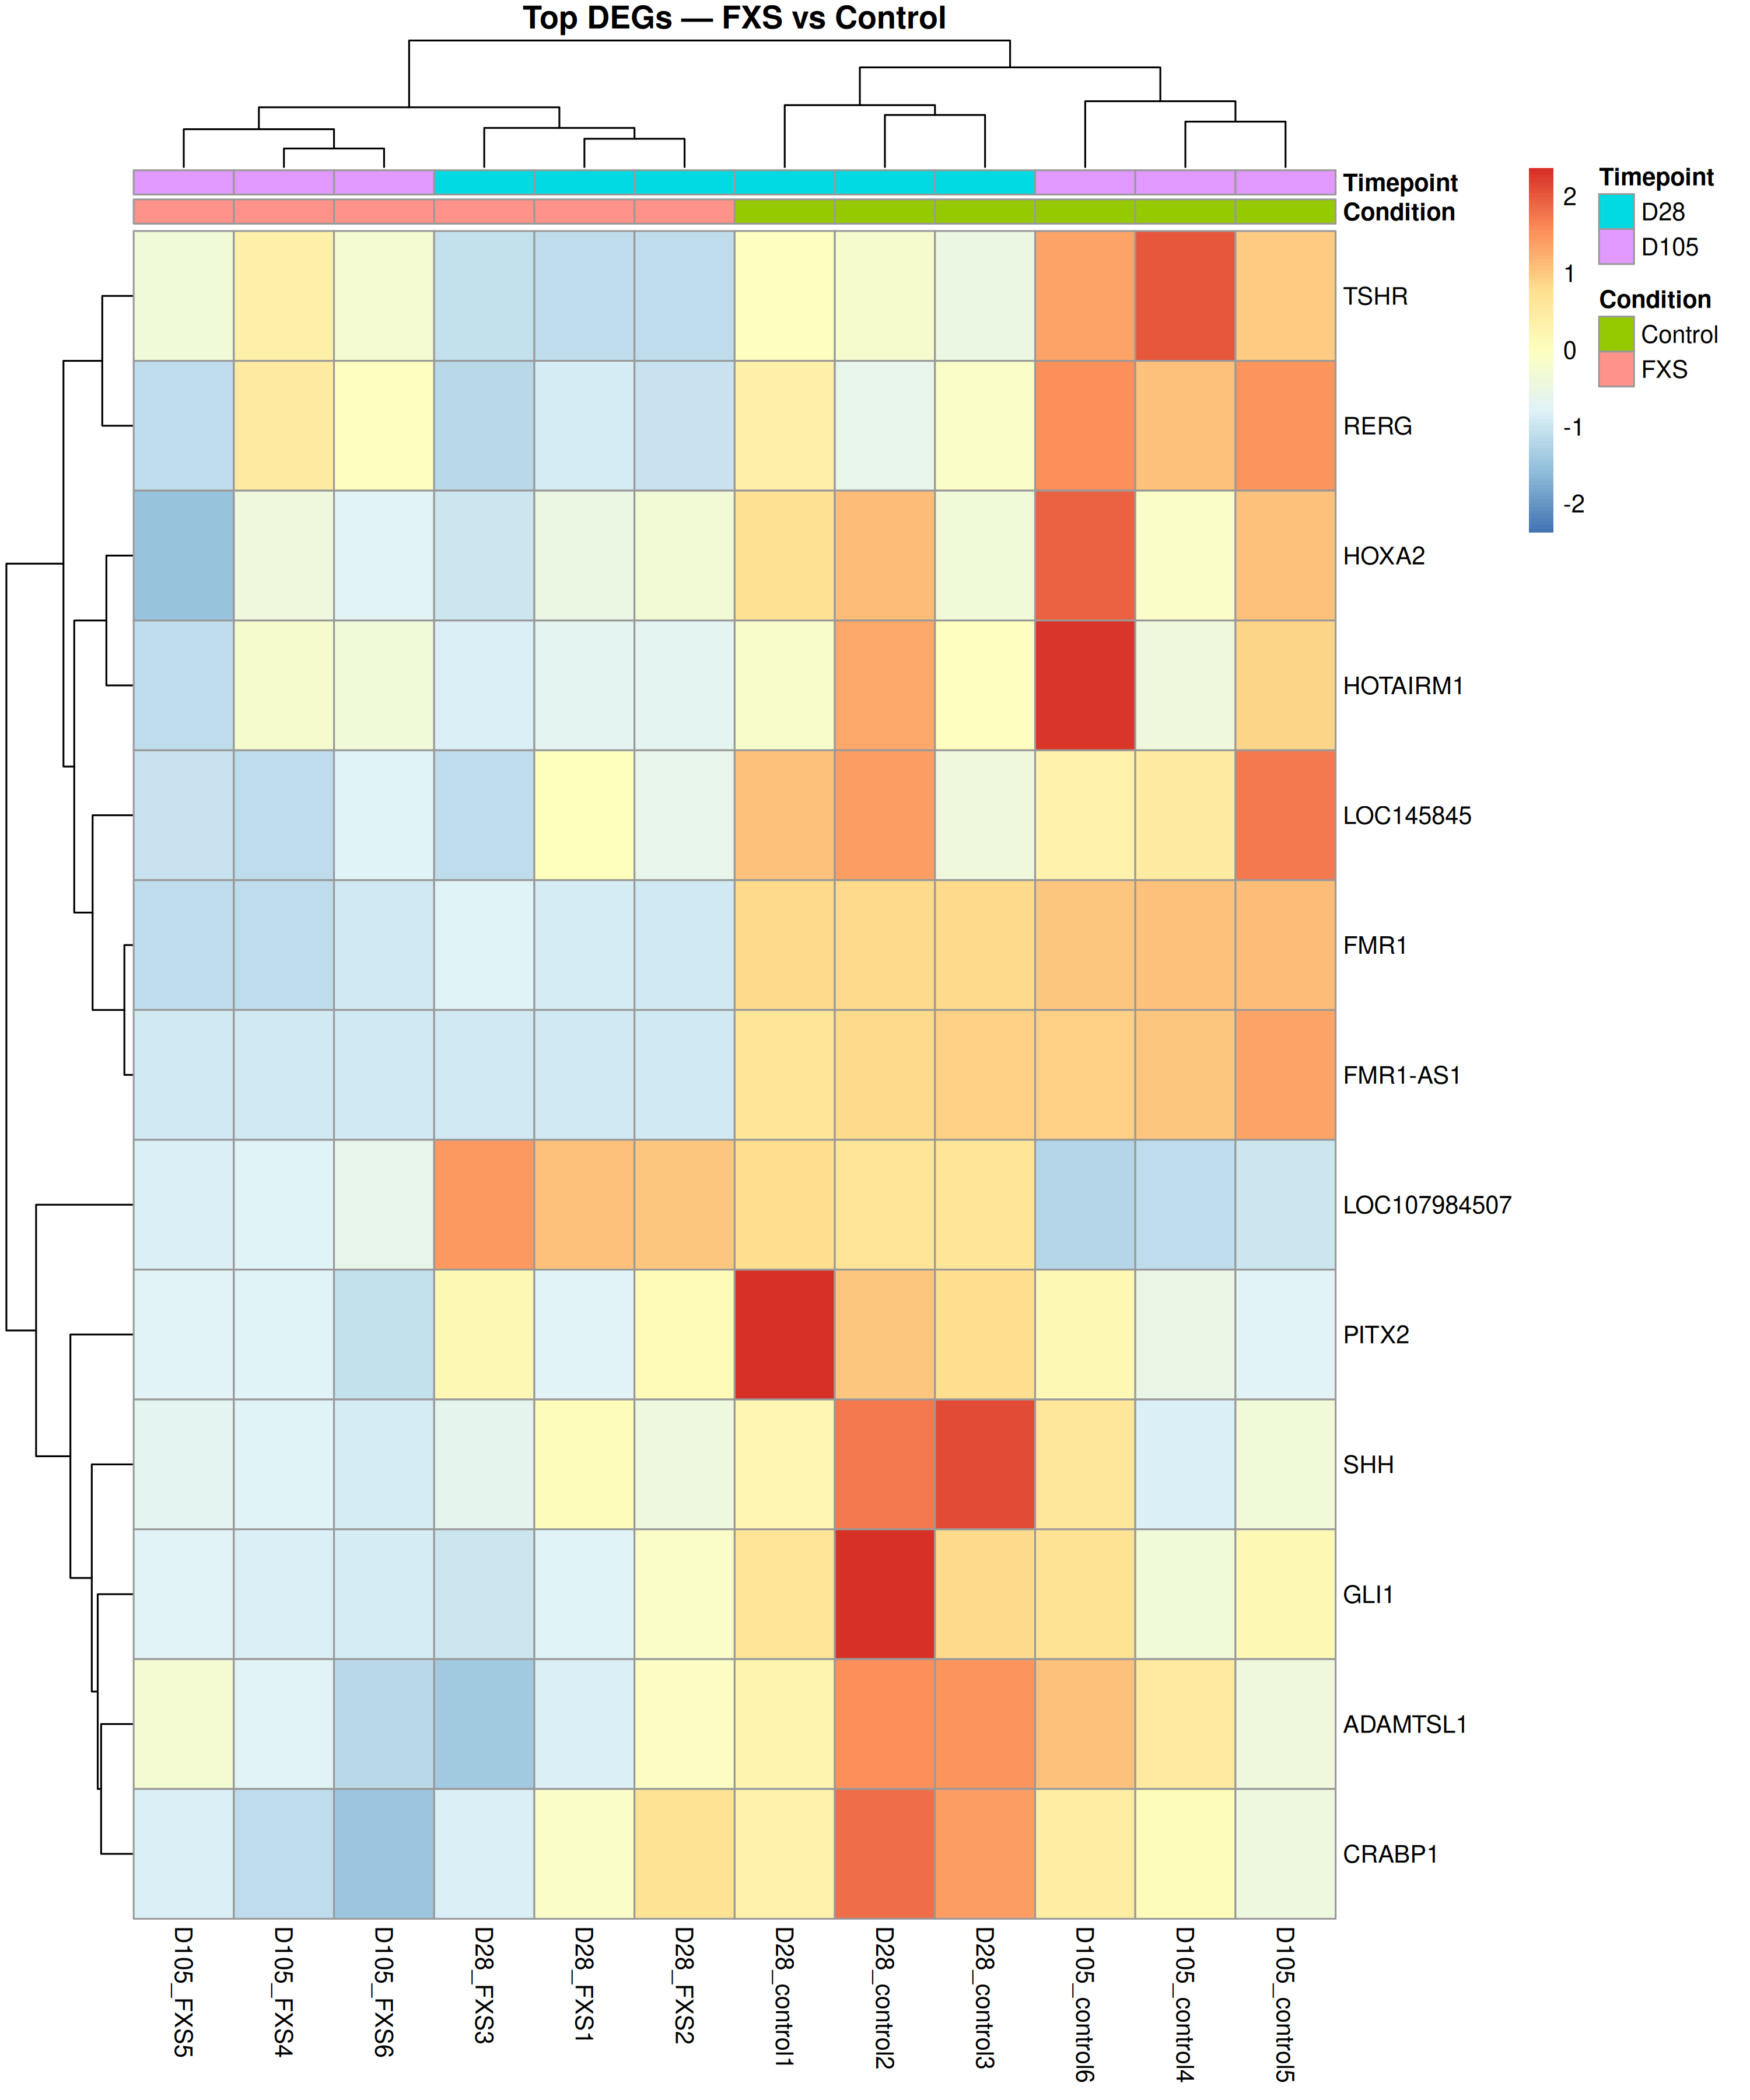
\includegraphics[width=\columnwidth]{heatmap_top_DEGs.png}
\caption{Heatmap of the top differentially expressed genes, GSE146339, led by \gene{FMR1} and \gene{FMR1-AS1}.}
\label{fig:heatmap}
\end{figure}

Differential methylation analysis found 25 significant DMPs mapping to 10 genes, with \gene{FMR1} and \gene{ASFMR1} showing by far the strongest hypermethylation signal (mean $\Delta\beta=0.56$ across 15 probes shared between the two genes)---consistent with the well-established mechanism of CGG-repeat-induced \gene{FMR1} silencing, and, notably, focal rather than genome-wide: of the remaining eight significant DMP genes, seven were hypomethylated and one (\gene{TRAF1}) was hypermethylated, all with modest effect sizes ($|\Delta\beta|$ between 0.11 and 0.21). As noted in the Introduction, this replication is an internal validity check rather than a new mechanistic claim; the continuous promoter-methylation weighting derived from it is what actually feeds forward into the PANDA prior (Section~IV-F, Fig.~\ref{fig:methweight}).

\begin{figure}[!t]
\centering
\twofig{methylation_gene_summary.png}{promoter_methylation_distribution.png}
\caption{Differential methylation summary. Left: differentially methylated genes, GSE41273 (FDR $<0.05$, $|\Delta\beta|>0.1$); \gene{FMR1} and \gene{ASFMR1} show the strongest hypermethylation signal. Right: distribution of promoter methylation used to derive the continuous PANDA accessibility prior.}
\label{fig:meth}
\end{figure}

\subsection{GENIE3 and PANDA Networks}
The GENIE3 network comprised 1,340 nodes and 173,517 edges after retaining the top decile of edge weights; the full PANDA network, restricted to genes with available promoter annotation, motif scans, and STRING PPI entries, comprised 2,841 nodes and 339,985 positive-score edges, of which the top decile by edge score (2,662 nodes, 33,999 edges) was retained for visualization and hub ranking (Fig.~\ref{fig:networks}; full networks in \repo{results/GENIE3/GENIE3_network.graphml} and \repo{results/PANDA/PANDA_edge_list.csv}).

\begin{figure}[!t]
\centering
\twofig{GENIE3_network_plot.png}{PANDA_network_plot.png}
\caption{Comparison of inferred TF regulatory networks. Left: GENIE3 (expression-only). Right: PANDA (motif + STRING PPI + methylation prior).}
\label{fig:networks}
\end{figure}

Ranking TFs by weighted out-degree in each network showed that none of the six a priori known FXS regulators appeared among the genome-wide top-50 hub TFs in either network (Fig.~\ref{fig:hubs}). This is not, on its own, evidence against their biological relevance: given the target-eligibility restriction described in Section~IV-D, only a small fraction of each TF's full motif regulon was ever eligible to be rediscovered in the first place.

\begin{figure}[!t]
\centering
\twofig{GENIE3_hub_genes.png}{PANDA_hub_genes.png}
\caption{Top hub TFs by weighted out-degree. Left: GENIE3. Right: PANDA. None of the six a priori reference TFs (SP1, NRF1, REST, FOXG1, SIX3, TFAP2A) appears in either top-50 list.}
\label{fig:hubs}
\end{figure}

\subsection{Permutation Nulls}
Results here motivate the more cautious framing of the rest of the paper. The GENIE3 permutation null found 46,796 edges nominally significant at $p<0.05$, but \textbf{zero} survived FDR $<0.05$. The PANDA randomized-prior null produced a 95th-percentile edge score ($q_{95}=3.49$) almost identical to the observed 90th-percentile threshold (3.51), indicating that PANDA edge scores largely reproduce the motif/PPI prior rather than adding expression-driven signal at this sample size (Fig.~\ref{fig:null}).

\begin{figure}[!t]
\centering
\twofig{GENIE3_null_distribution.png}{PANDA_null_distribution.png}
\caption{Permutation null distributions used to FDR-correct network edges. Left: GENIE3 label-shuffled null. Right: PANDA randomized-prior null.}
\label{fig:null}
\end{figure}

The ALPACA permutation null found 484 nodes nominally significant, again \textbf{zero} surviving FDR correction, with the best-performing of the nine candidate modules (module 1, 113 nodes) reaching only module-level FDR $=0.19$ (Fig.~\ref{fig:alpaca}; \repo{results/ALPACA/ALPACA_module_significance.csv}).

\subsection{Sample-Specific Networks and Bootstrap Test}
LIONESS produced 12 sample-specific networks (one per RNA-seq sample in the primary cohort). Across all TF--target interactions, 49.9\% of edges were stronger in FXS than in the mean control network (bootstrap 95\% CI: [46.7\%, 52.3\%]; \repo{results/LIONESS/LIONESS_bootstrap_CI.csv})---a confidence interval that straddles 50\%, i.e.\ no systematic genome-wide shift in regulatory strength toward either condition is statistically supported by this test (Fig.~\ref{fig:boot}). The top individual edges by FXS-vs-control weight difference and the activity of the six a priori reference TFs across samples are shown in Fig.~\ref{fig:lion}, and the per-edge comparison in Fig.~\ref{fig:lionscatter}.

\begin{figure}[!t]
\centering
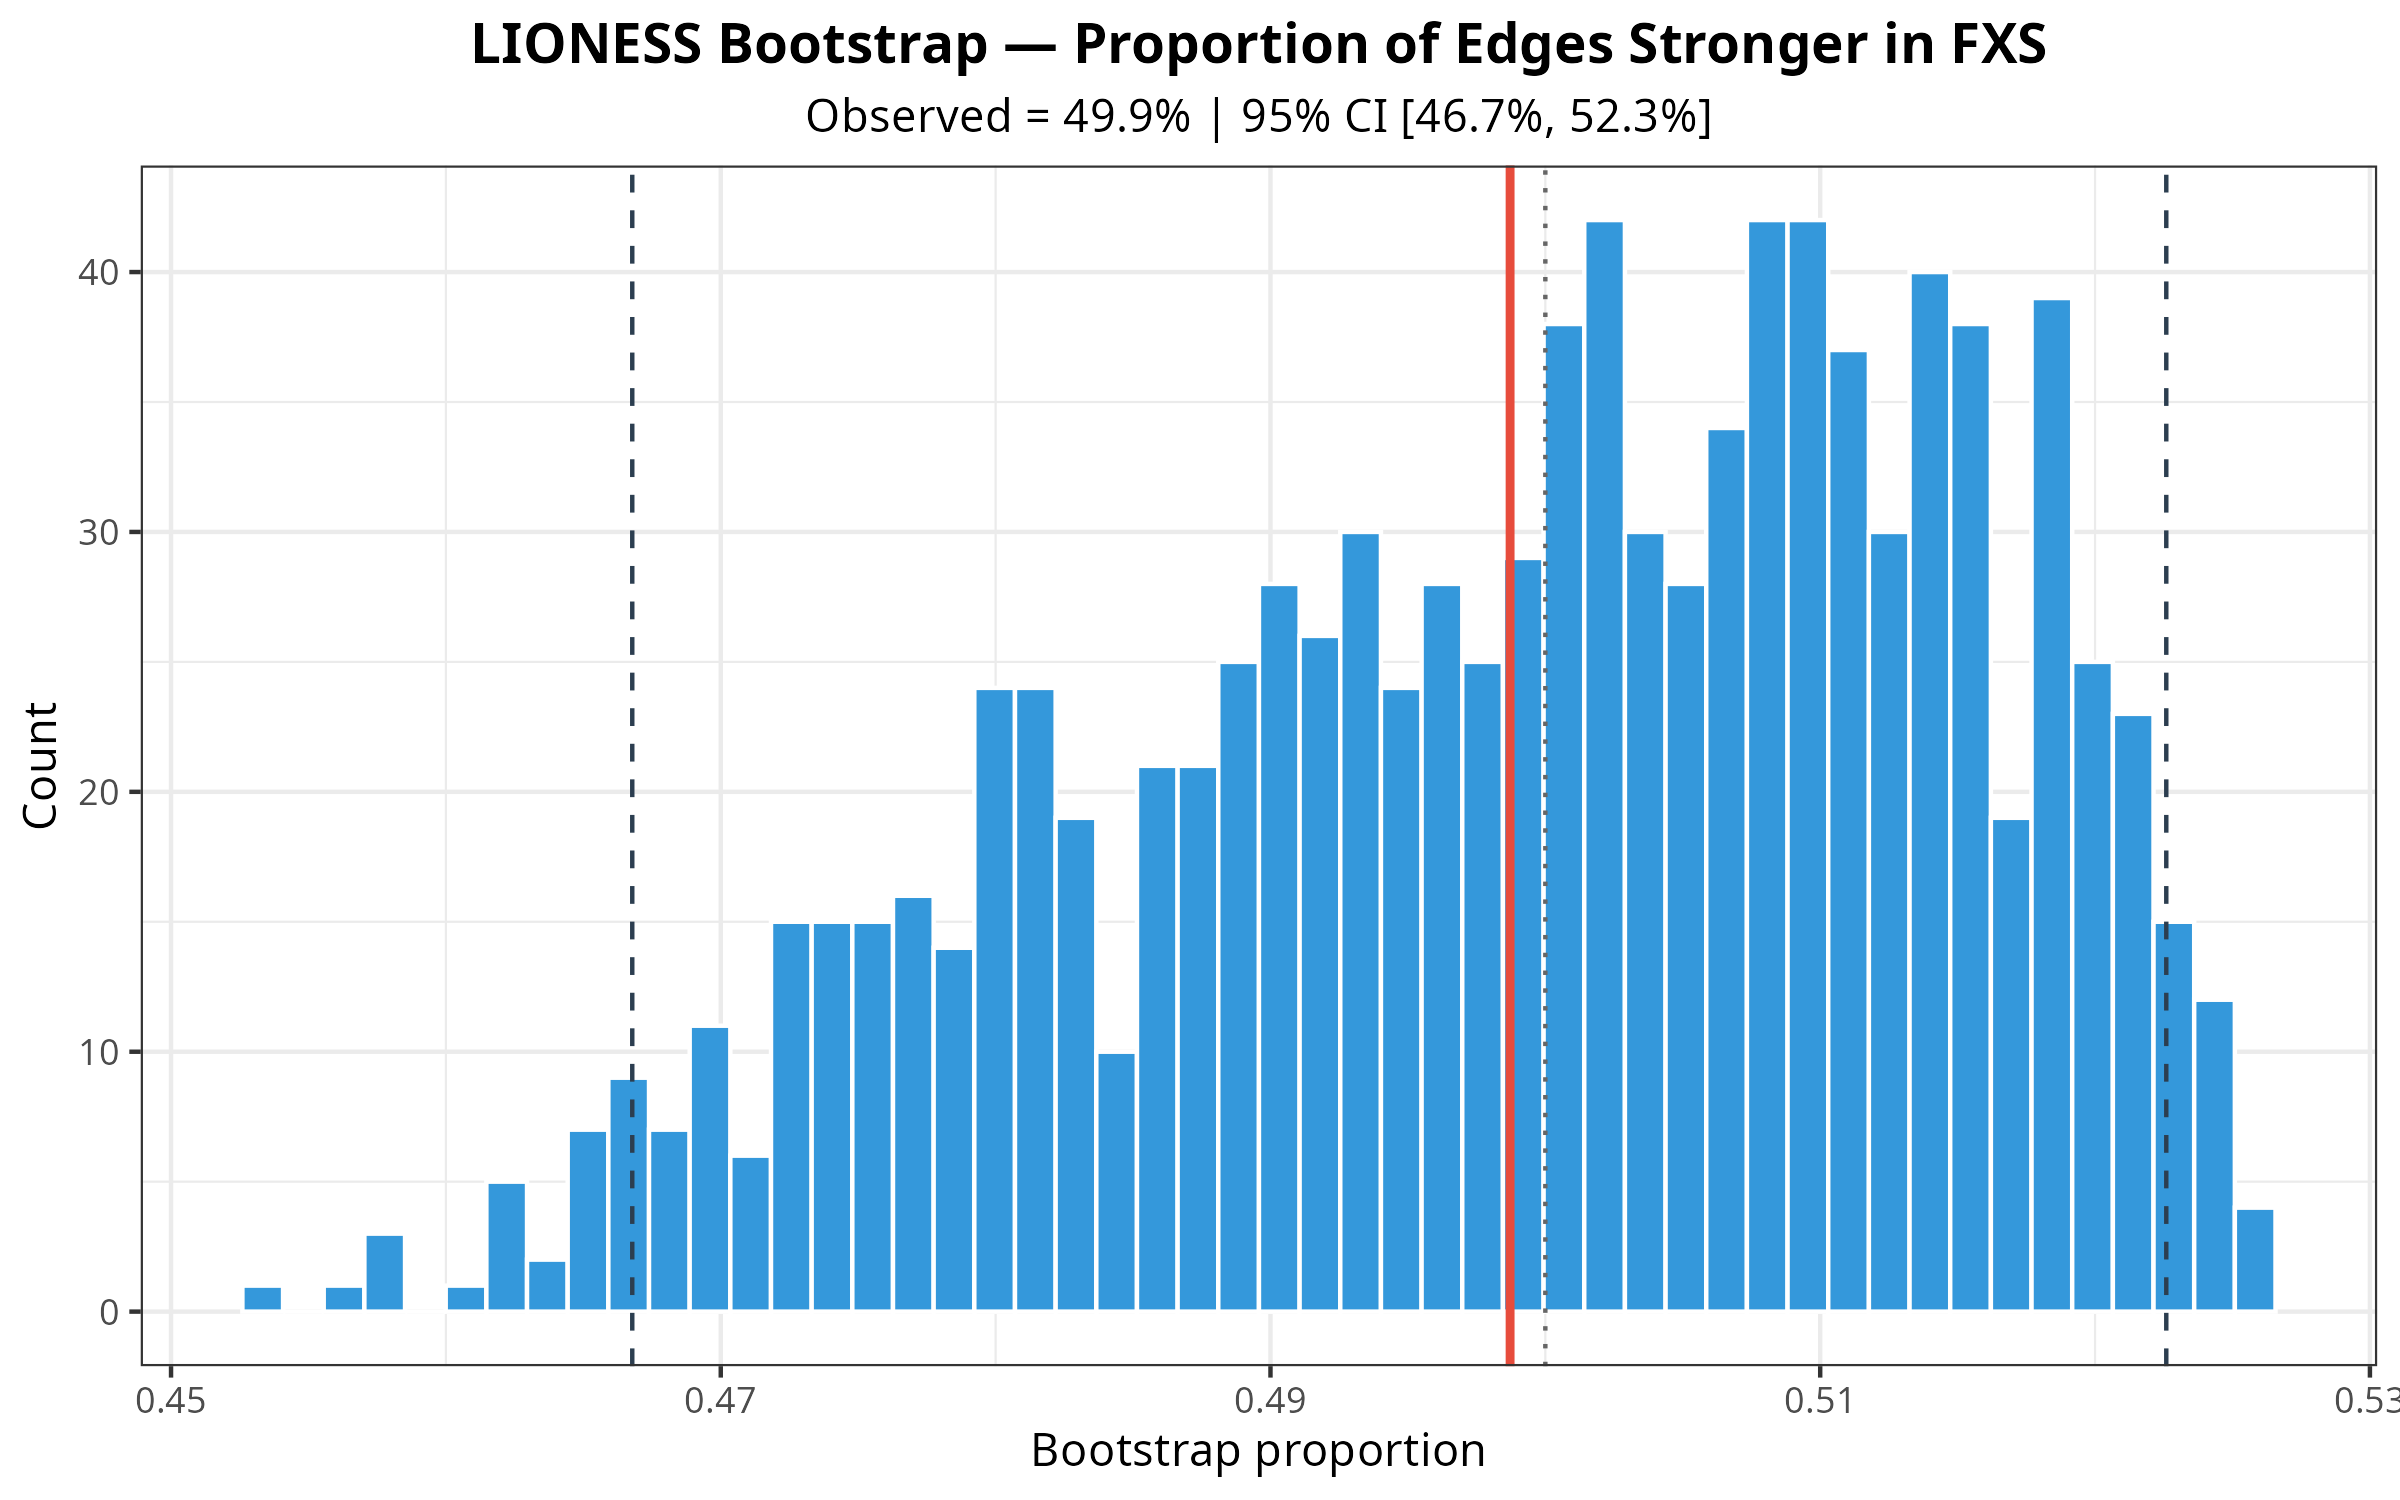
\includegraphics[width=\columnwidth]{LIONESS_bootstrap_distribution.png}
\caption{LIONESS sample-specific network bootstrap test: distribution of the proportion of edges stronger in FXS than in the mean control network across 1,000 resamples. The 95\% CI straddles 50\%.}
\label{fig:boot}
\end{figure}

\begin{figure}[!t]
\centering
\twofig{LIONESS_top_edges_barplot.png}{LIONESS_known_TF_activity.png}
\caption{LIONESS sample-specific network detail. Left: top individual TF--target edges ranked by FXS-vs-control weight difference. Right: sample-specific activity of the six a priori reference TFs.}
\label{fig:lion}
\end{figure}

\begin{figure}[!t]
\centering
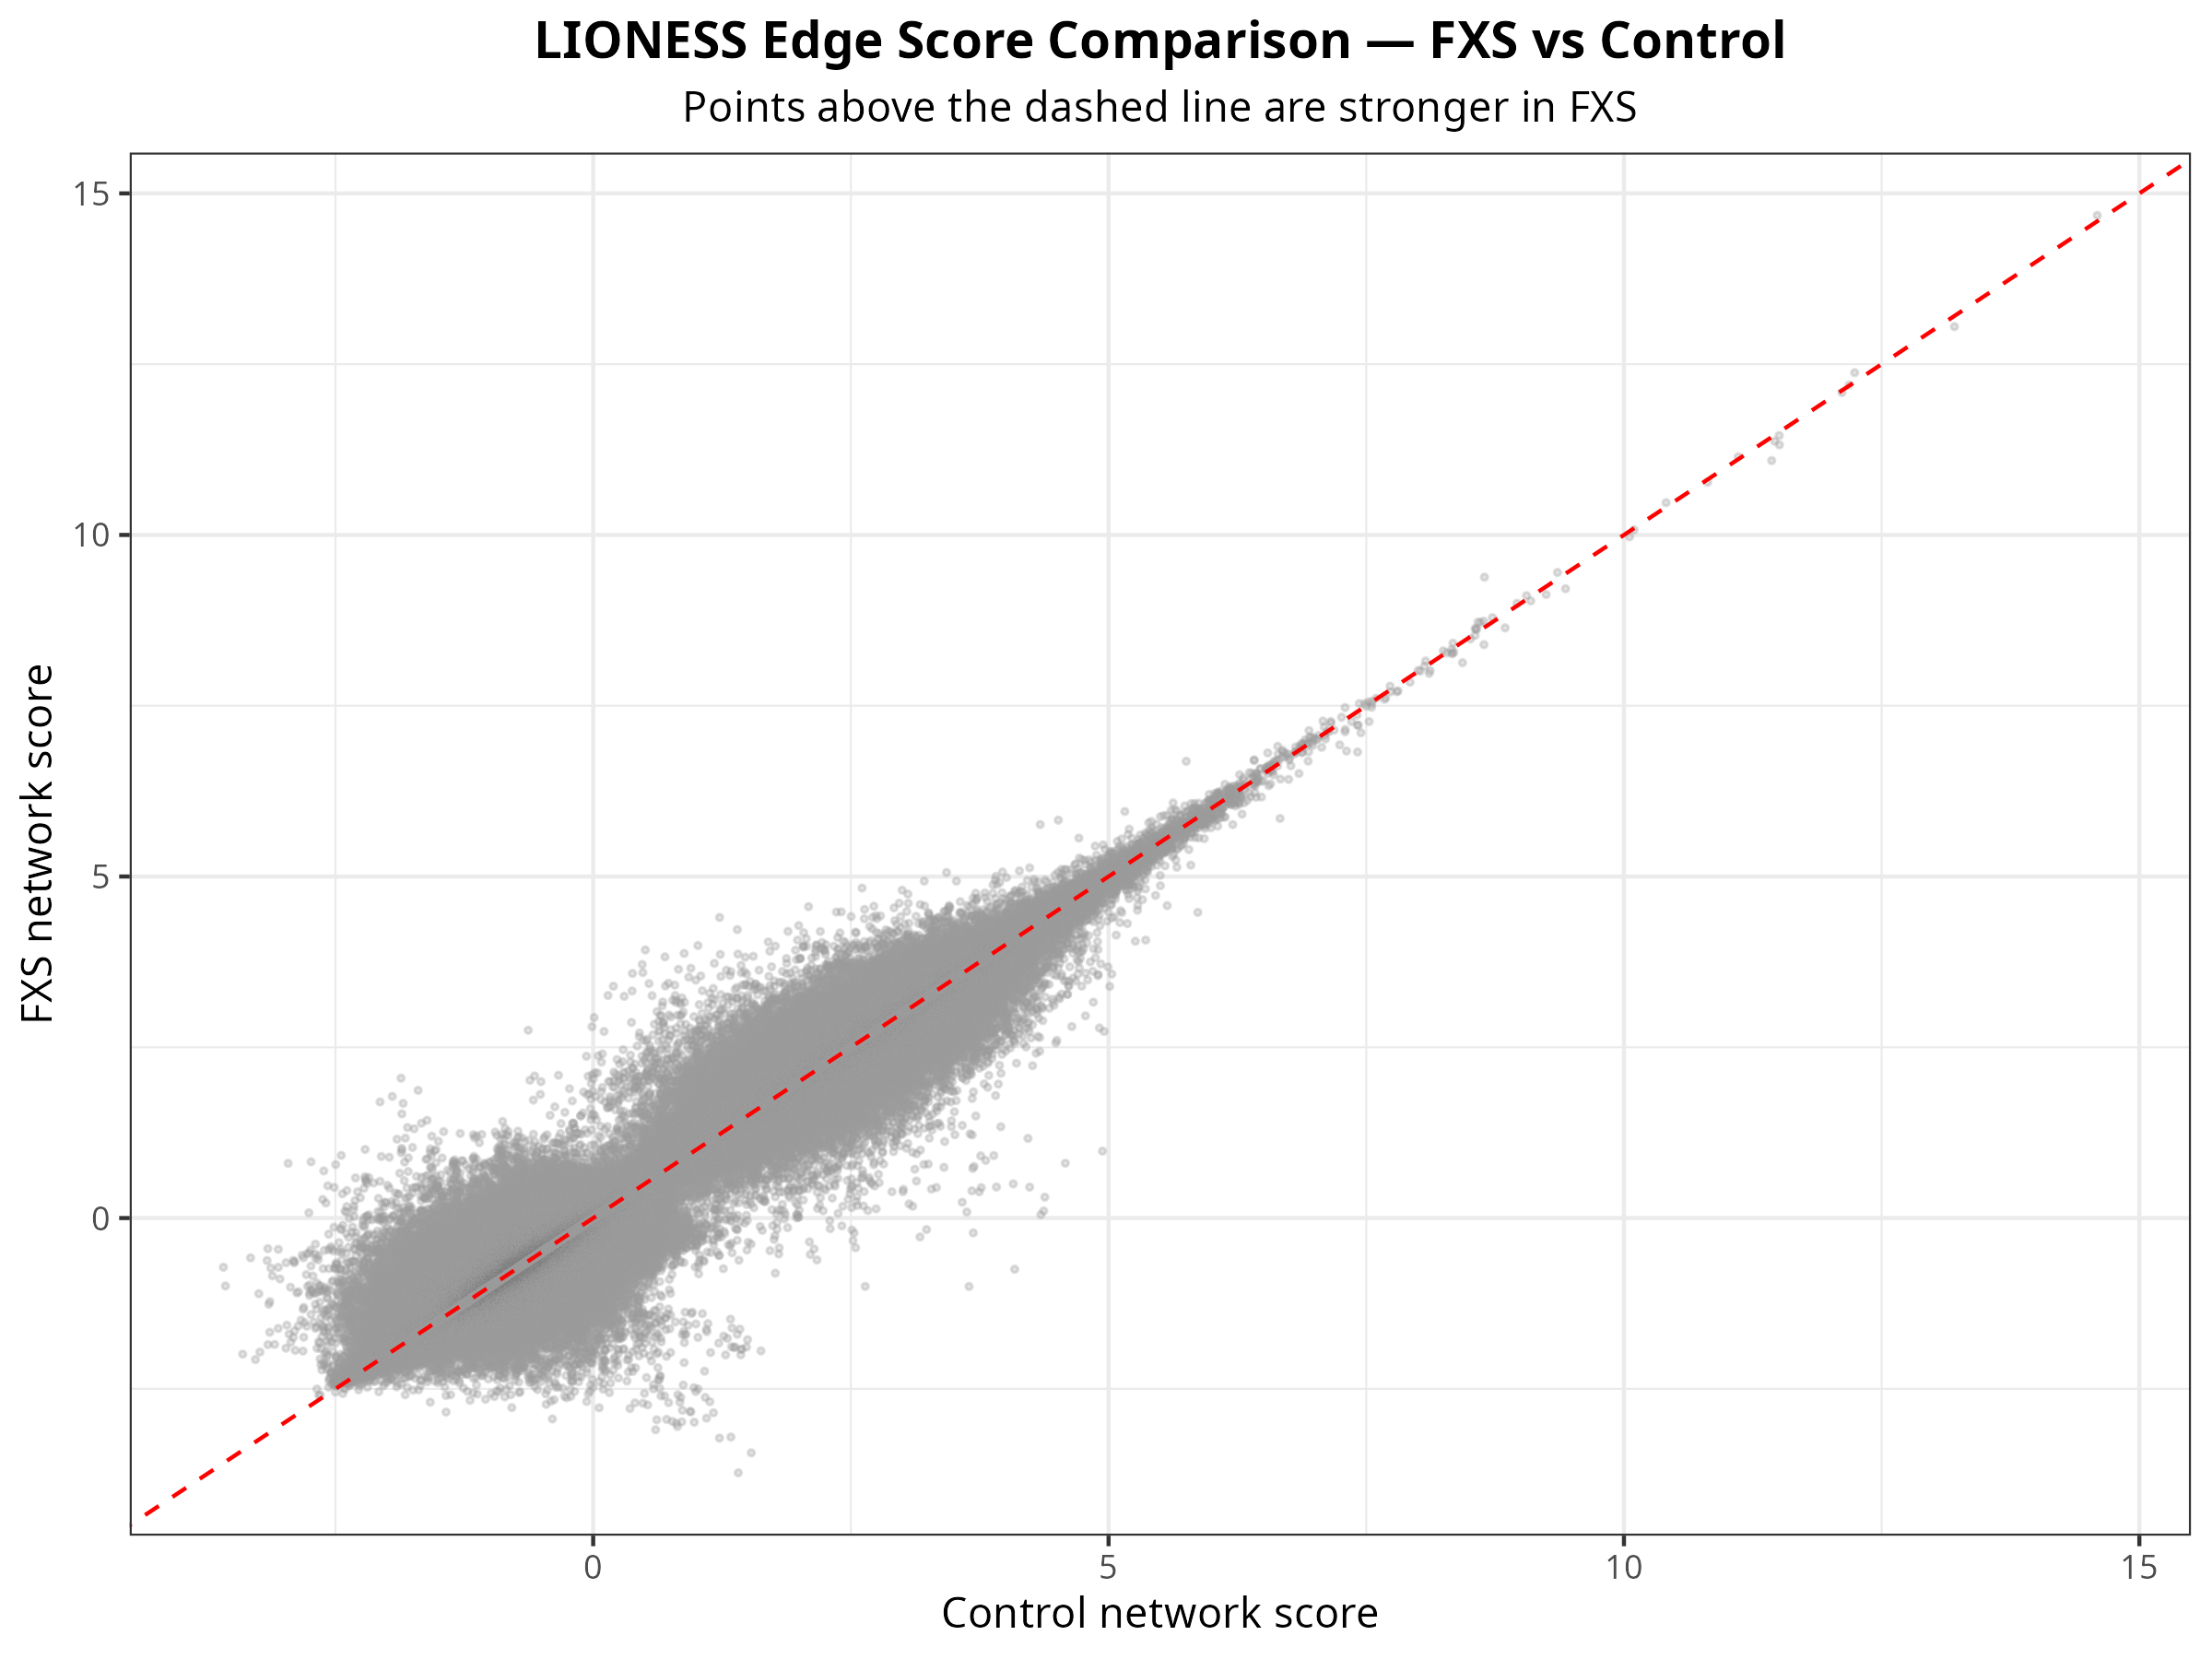
\includegraphics[width=\columnwidth]{LIONESS_FXS_vs_Control_scatter.png}
\caption{Per-edge LIONESS weight in FXS vs.\ control aggregate networks; the near-diagonal scatter reflects the absence of a systematic genome-wide shift reported above.}
\label{fig:lionscatter}
\end{figure}

\subsection{Cross-Cohort Validation}
Genome-wide effect-size correlation between the two RNA-seq cohorts was weak (Pearson $r=0.034$, $p=3.0\times10^{-8}$; Spearman $\rho=0.024$, $p=7.2\times10^{-5}$), and sign concordance across all 27,072 shared genes was 50.6\%---indistinguishable from chance (Fig.~\ref{fig:conc}; \repo{results/validation/crossvalidation_concordance_summary.csv}).

\begin{figure}[!t]
\centering
\twofig{crossvalidation_global_LFC_correlation.png}{crossvalidation_direction_concordance.png}
\caption{Cross-cohort concordance detail. Left: genome-wide effect-size correlation across all 27,072 shared genes ($r=0.034$; genome-wide sign concordance 50.6\%, indistinguishable from chance). Right: direction of change for the DEG shared by both cohorts---only \gene{FMR1}, which is concordantly downregulated (1/1).}
\label{fig:conc}
\end{figure}

RRHO2 nonetheless detected a significant peak of rank--rank overlap ($-\log_{10}p=14.07$), suggesting some concordant structure exists in a subset of the ranked gene lists even though it does not show up as a genome-wide linear correlation. An independent re-implementation of the original RRHO grid on the same 27,072 genes gave a comparable peak ($-\log_{10}p=13.45$; Fig.~\ref{fig:rrhomanual}); in both, the peak lies at large rank cutoffs, i.e.\ in the broad body of the ranked lists rather than among the top-ranked genes. At the level of individual DEGs, only \gene{FMR1} itself was shared between the primary (13 DEGs) and validation (63 DEGs, of which 22 are measured in both cohorts and therefore enter the overlap test) significant sets, but this single-gene overlap was $94.7\times$ enriched over the chance expectation given the small DEG set sizes (hypergeometric $p=0.0105$; Fisher OR $=107$; \repo{results/validation/crossvalidation_overlap_significance.csv}).

\begin{figure}[!t]
\centering
\twofig{crossvalidation_venn.png}{RRHO2_heatmap.png}
\caption{Cross-cohort validation between GSE146339 and GSE218676. Left: DEG overlap---only \gene{FMR1} is shared between the two significant sets. Right: RRHO2 rank--rank overlap heatmap.}
\label{fig:venn}
\end{figure}

\begin{figure}[!t]
\centering
\includegraphics[width=\columnwidth]{RRHO_manual_twocohort.png}
\caption{Independent RRHO cross-check on the two RNA-seq cohorts (GSE146339 vs.\ GSE218676; 27,072 jointly measured genes ranked by signed $-\log_{10}p$; $99\times99$ grid). The peak ($-\log_{10}p=13.45$) agrees with the RRHO2 result in Fig.~\ref{fig:venn}.}
\label{fig:rrhomanual}
\end{figure}

\subsection{Tissue-General versus Tissue-Specific Effects}
Applying the classification defined in Section~IV-J across all three tissue contexts, \gene{FMR1} was the only gene called tissue-general under the $\geq$2-of-3 rule, appearing as a significant DEG in both RNA-seq cohorts (Section~V-A) and among the strongest hypermethylation signals in the methylation cohort through the 15 probes in its shared promoter with \gene{ASFMR1}. Of 83 genes reaching significance in exactly one tissue context, 12 were specific to the primary organoid cohort, 62 to the validation NPC/B-lymphocyte/iPSC cohort, and 9 to the methylation cohort alone. No gene was significant in all three contexts simultaneously except \gene{FMR1}.

This pattern is consistent with, rather than contradictory to, the weak genome-wide cross-cohort correlation reported above: almost all detectable transcriptional and epigenetic change downstream of \gene{FMR1} silencing appears to be tissue-restricted, with the causal lesion itself as the one clear exception.

\subsection{Functional Enrichment of ALPACA Modules}
ALPACA identified nine candidate differential modules of varying size (113--560 nodes), none reaching genome-wide significance against the permuted null (Figs.~\ref{fig:alpaca}--\ref{fig:alpacanet}; module memberships and scores in \repo{results/ALPACA/}).

\begin{figure}[!t]
\centering
\twofig{ALPACA_module_sizes.png}{ALPACA_module_significance.png}
\caption{ALPACA differential modularity. Left: size of each of the nine candidate modules. Right: module significance vs.\ the permuted null---the best module reaches only FDR $=0.19$.}
\label{fig:alpaca}
\end{figure}

\begin{figure}[!t]
\centering
\twofig{ALPACA_top_nodes.png}{ALPACA_FXS_TF_modules.png}
\caption{Left: top nodes by differential modularity contribution. Right: the six a priori reference TFs mapped onto their ALPACA modules.}
\label{fig:alpacanodes}
\end{figure}

\begin{figure}[!t]
\centering
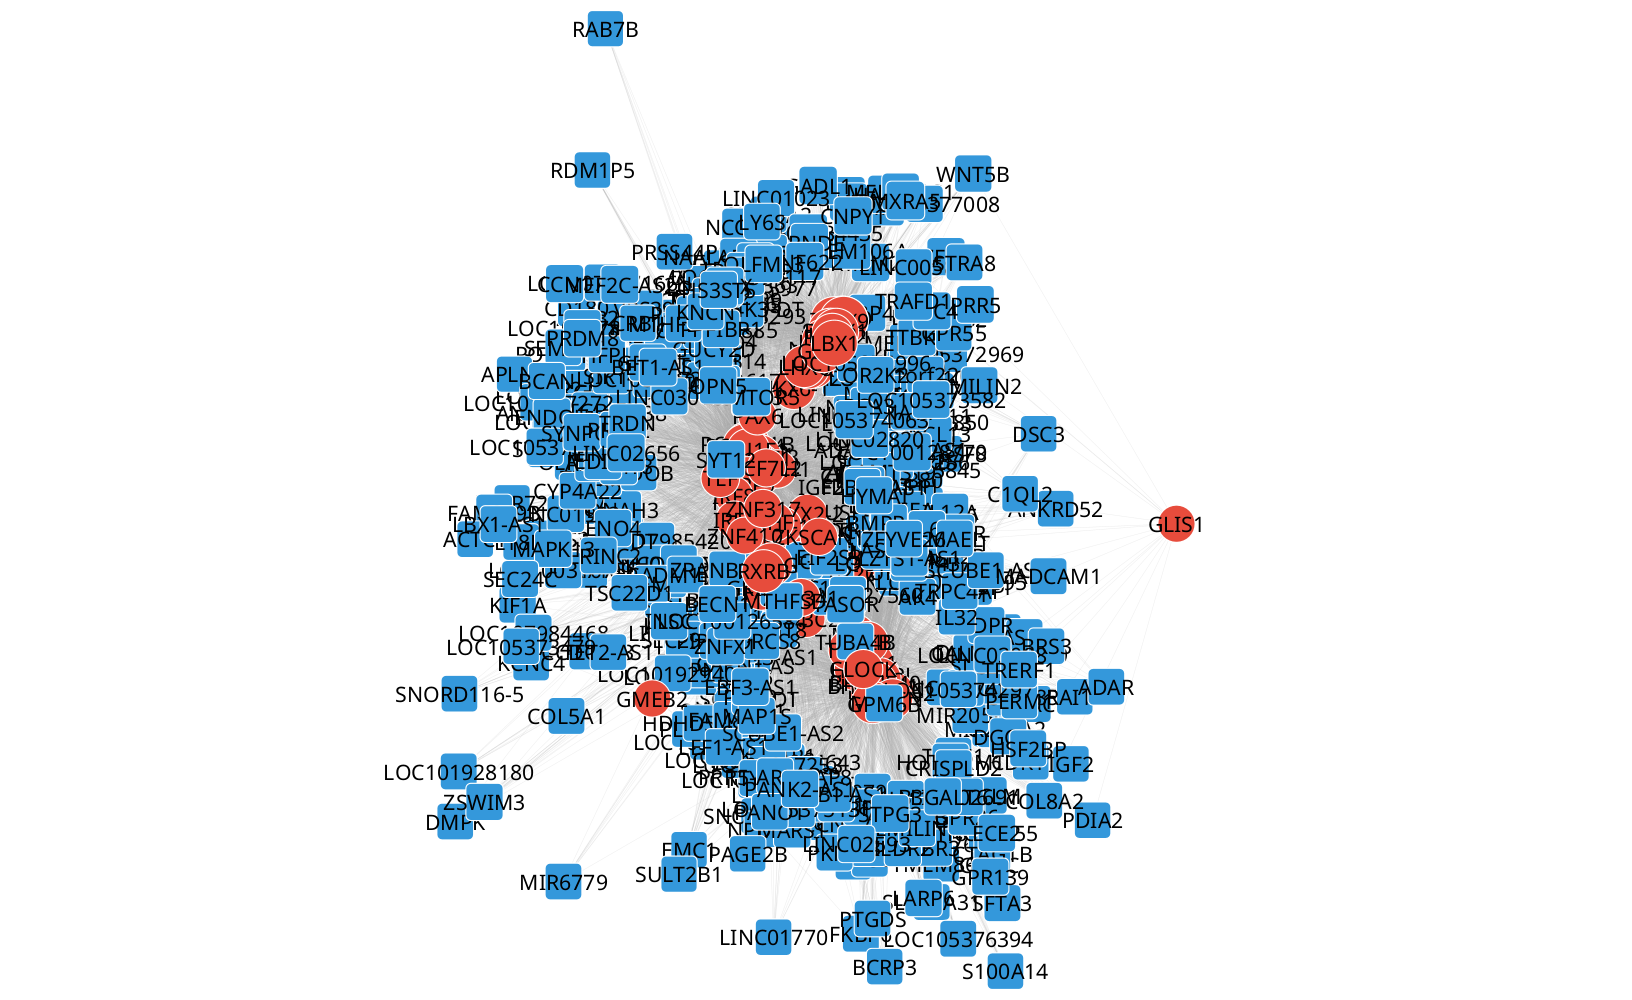
\includegraphics[width=\columnwidth]{FXS_ALPACA_network_final.png}
\caption[ALPACA network]{Final annotated ALPACA differential-module network for FXS, visualized in Cytoscape~\cite{cytoscape} (\repo{networks/FXS_ALPACA_network.xgmml}).}
\label{fig:alpacanet}
\end{figure}

At the strict threshold (FDR $<0.05$), GO Biological Process enrichment of the ALPACA differential-module genes returned terms centered on nervous system development, positive and negative regulation of DNA-templated transcription, and RNA polymerase II transcriptional regulation, driven substantially by forkhead-box (\gene{FOXA2, FOXA3, FOXK1, FOXK2, FOXO3, FOXO4, FOXP1, FOXP3}) and HES/HEY family genes (Fig.~\ref{fig:go}; \repo{results/ALPACA/ALPACA_module_GO_enrichment.csv}).

\begin{figure}[!t]
\centering
\twofig{ALPACA_module_GO_dotplot.png}{ALPACA_topHits_GO_dotplot.png}
\caption{GO Biological Process enrichment of ALPACA differential modules. Left: all modules, strict threshold (FDR $<0.05$). Right: top-hit genes only.}
\label{fig:go}
\end{figure}

At the relaxed threshold, KEGG pathway enrichment surfaced FoxO signaling, Notch signaling, and Polycomb repressive complex terms, alongside several broader cancer- and cell-cycle-associated pathways that likely reflect shared proliferation/differentiation biology rather than anything FXS-specific (Fig.~\ref{fig:kegg}; \repo{results/ALPACA/ALPACA_topHits_KEGG_relaxed.csv}).

\begin{figure}[!t]
\centering
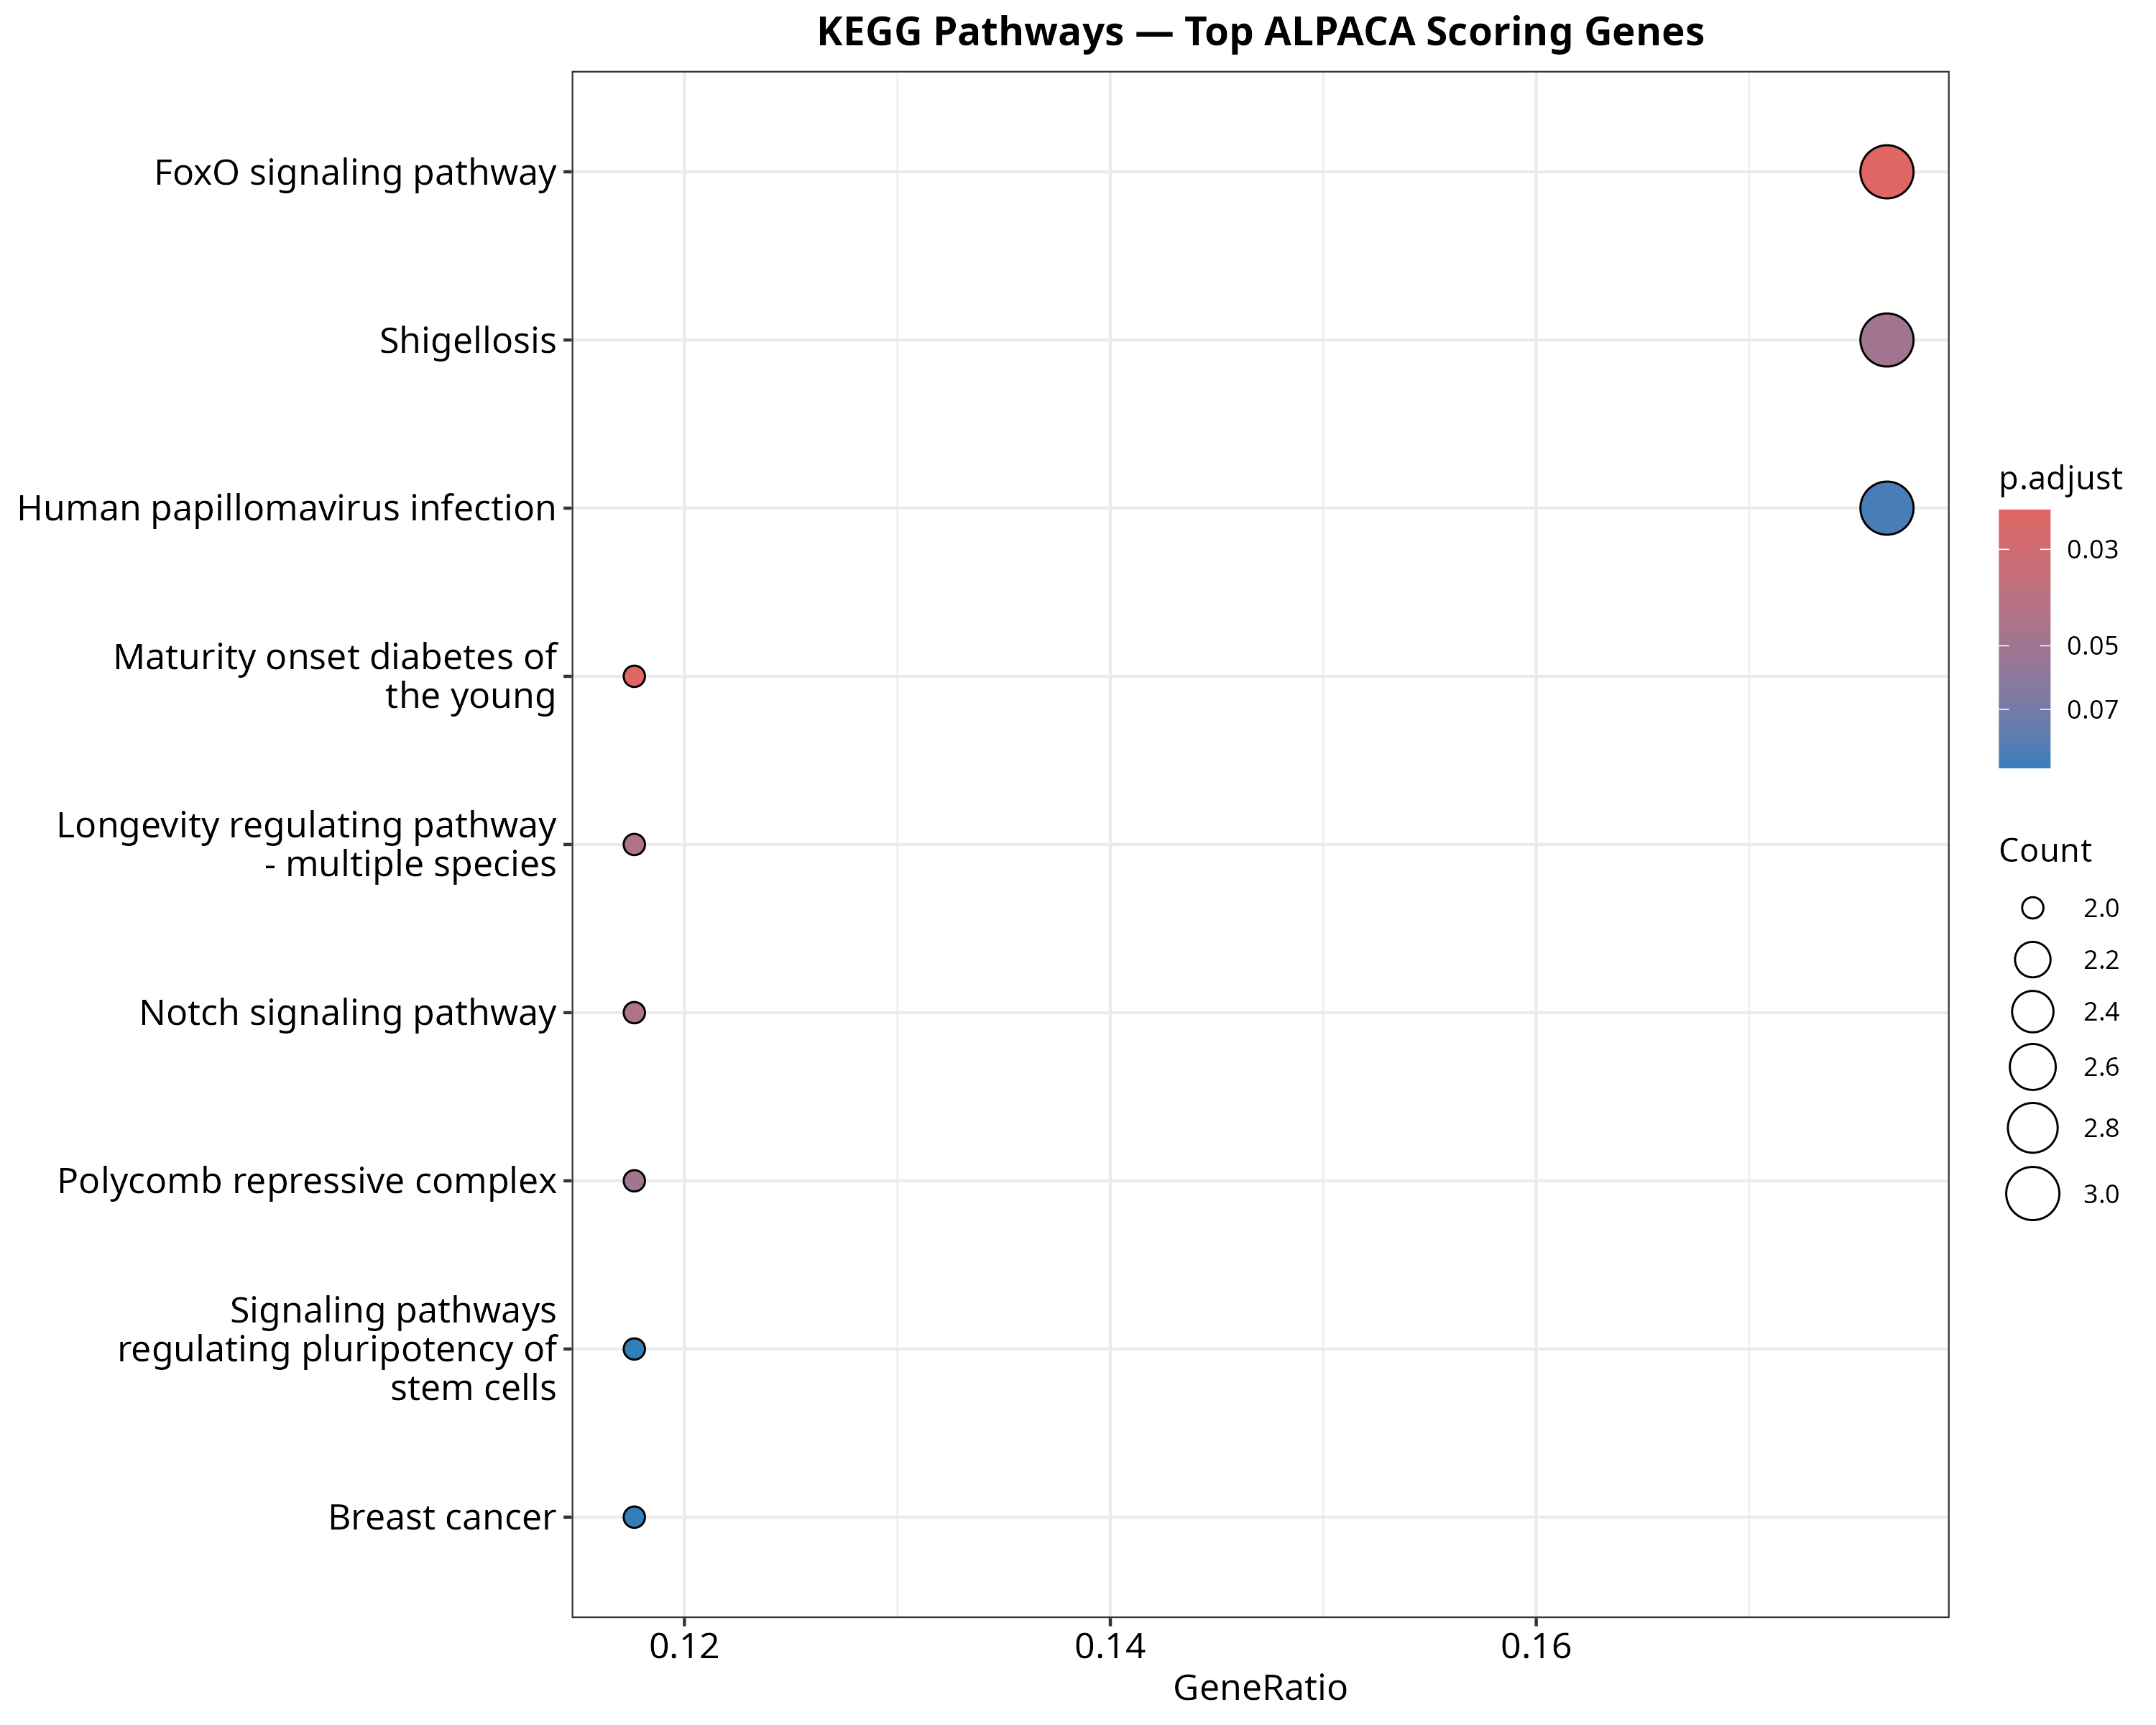
\includegraphics[width=\columnwidth]{ALPACA_topHits_KEGG_dotplot.png}
\caption{KEGG pathway enrichment of ALPACA top-hit genes at the relaxed threshold (nominal $p<0.1$), surfacing FoxO signaling, Notch signaling, and Polycomb repressive complex terms.}
\label{fig:kegg}
\end{figure}

\subsection{In Silico Regulator Validation}
ENCODE ChIP-seq self-recovery was evaluated for 18 TF--network-source pairs (nine candidate TFs, each with a GENIE3- and a PANDA-derived target set; \repo{results/validation/ChEA3_ENCODE_selfrecovery.csv}). REST and NRF1 ranked 1 of 200 candidate regulators (PANDA-derived target sets), and SP1 ranked 5 (GENIE3) and 14 (PANDA). Across the 18 pairs, 6 ranked $\leq10$ and 9 ranked $\leq25$.

TRRUST curated-target enrichment was evaluated separately for 20 TF--network-source pairs (the ten candidate TFs with curated targets in TRRUST, each with both target sets; \repo{results/validation/TRRUST_validation_results.csv}). Three of the 20 pairs cleared FDR $<0.05$, all from GENIE3-derived target sets: SP1 ($4.3\times$ enrichment, 17 overlapping targets, FDR $=3.5\times10^{-6}$), HOXA10 and HOXA9 (both $\approx10.7$--$10.9\times$, FDR $=0.012$, each resting on only three overlapping targets). SP1 with PANDA-derived targets (FDR $=0.090$) and TFAP2A with GENIE3-derived targets (FDR $=0.088$) were nominally enriched only.

\begin{figure}[!t]
\centering
\twofig{FXS_TF_OutDegree_comparison.png}{known_TF_module_local_centrality.png}
\caption[Hub vs local centrality]{Genome-wide hub status vs.\ module-local relevance for the six a priori reference TFs. Left: weighted out-degree, genome-wide (none rank as top hubs). Right: within-module edge strength (SP1, REST, and NRF1 rank at the 90th--96th percentile of module 7; FOXG1 and TFAP2A rank similarly within module 9; \repo{results/ALPACA/ALPACA_module_local_centrality.csv}).}
\label{fig:local}
\end{figure}

Fig.~\ref{fig:local} shows the comparison underlying the ``locally central but not a genome-wide hub'' pattern discussed next.

\section{Discussion}
Taken together, these results support a narrower and more specific claim than the framework was originally built to test. \gene{FMR1} silencing itself replicates essentially perfectly across three independent datasets and three tissue contexts, which is reassuring but unsurprising---it is, after all, the causal lesion, and its hypermethylation-to-silencing mechanism was already established by prior work~\cite{peprah2012,hayward2021,liu2018,brykczynska2016} rather than something this paper set out to discover. What does not replicate cleanly is genome-wide regulatory rewiring downstream of that lesion: cross-cohort effect-size correlation is close to zero, the LIONESS bootstrap interval straddles 50\%, and every permutation null we ran for GENIE3, PANDA, and ALPACA came back empty at genome-wide significance. Read alongside the tissue-generality classification in Section~V-F, this weak correlation looks less like a failure of the pipeline and more like a substantive finding in its own right: almost every downstream effect we detect is restricted to a single tissue context, and \gene{FMR1} is the sole exception. A near-zero genome-wide correlation is close to what that picture would predict, so we treat it here as evidence for tissue-specific downstream regulation rather than purely as a limitation of statistical power---though we cannot fully separate the two explanations with only two RNA-seq cohorts, a point we return to in Limitations. The same logic extends to the methylation result in Section~V-A: the fact that hypermethylation was tightly focal to \gene{FMR1/ASFMR1} while the other eight significant DMP genes showed only modest changes is another instance of the same pattern, not a separate anomaly.

We think the more interesting result sits underneath those negative network-level tests: several regulators with prior FXS literature support---especially SP1, REST, and NRF1---show up as locally central within their own ALPACA module (Fig.~\ref{fig:local}; 90th--96th percentile of within-module edge strength) and are independently recoverable from ENCODE ChIP-seq and TRRUST evidence, even though none of them are genome-wide network hubs and even though the permutation null says the network as a whole is not distinguishable from noise. Two caveats apply: all three fall in the same module (module 7), which itself has no differential-modularity support against the null (module FDR $=1$), and FOXG1 and TFAP2A reach similarly high within-module strength (module 9) without the same in silico support, so local centrality alone does not single out these regulators. That combination is what one would expect if the true signal is real but concentrated in a handful of TFs, sitting inside a network whose bulk edge structure genuinely is underpowered at $n=6$ vs.\ $n=6$. The TRRUST enrichments for HOXA9 and HOXA10 pass FDR but rest on three overlapping targets each, so we regard them as weaker evidence than the SP1 result. Reporting only the module-level or hub-level finding, without the permutation null showing the rest of the network is noise, would have overstated what this dataset can support.

The significant RRHO peak alongside near-chance sign concordance is worth flagging as a general lesson for small-cohort regulatory genomics: aggregate correlation statistics and rank-based overlap statistics can disagree, and neither one alone tells the whole story about whether two cohorts ``agree.''

\section{Limitations}
A few constraints bound the scope of these results:
\begin{itemize}
\item \textbf{Tissue design.} The two RNA-seq cohorts differ in tissue composition, and methylation comes from a third, non-overlapping, unmatched cohort. We treat this as a designed tissue-generality comparison (Sections~IV-J, V-F), not a confound---but a gene called tissue-specific may just be under-detected elsewhere, not biologically absent.
\item \textbf{Methylation is a prior, not multi-omics.} With no subject overlap across cohorts, methylation informs the PANDA prior at the population level only; it cannot be linked to any individual's transcriptional response.
\item \textbf{GENIE3 target coverage.} 1,330 of the 1,340 eligible genes are themselves TFs, so the network is closer to a TF--TF map than a genome-wide TF--target map.
\item \textbf{Unmodeled covariates.} LIONESS does not adjust for developmental timepoint in the primary cohort, and two validation-cohort donors each contribute two cell types, modestly reducing effective sample size.
\item \textbf{In silico validation scope.} ENCODE/TRRUST enrichment shows inferred edges align with known TF--target binding above chance; it supports plausibility, not causal confirmation.
\end{itemize}
These reflect the general difficulty of network inference in a rare monogenic disorder with small public cohorts, and are reported alongside explicit permutation testing (Section~V-C) so readers can see which conclusions are well powered (\gene{FMR1} silencing, SP1/REST/NRF1 validation) and which are preliminary (genome-wide network topology).

\section{Future Work}
The most direct next step is validating this framework on larger, better-powered FXS cohorts as they become publicly available, which would let the permutation-null tests here actually pass rather than only bound the false-discovery rate at zero. Single-cell and spatial transcriptomic data would let cell-type-specific regulatory rewiring be characterized at a resolution bulk RNA-seq cannot reach. On the methods side, tighter integration of methylation into the motif prior (beyond the current continuous promoter-accessibility weighting), a systematic sensitivity analysis across network-inference thresholds, and comparison against other GRN methods such as ARACNe and GRNBoost2 would all help establish how much of the reported structure is method-specific. Extending the tissue-generality classification in Section~IV-J to matched, per-subject multi-omic cohorts---rather than the three independent, non-overlapping cohorts used here---would let us separate genuine tissue-specificity from cross-cohort noise more cleanly. Finally, experimentally validating SP1, REST, and NRF1---the three regulators that survive both local-centrality and in silico validation checks here---through CRISPR interference, reporter assays, or chromatin immunoprecipitation would be the most direct way to move these findings from hypothesis-generating to confirmatory.

\section{Conclusion}
This work builds a computational gene regulatory network framework for Fragile X syndrome that combines RNA-seq differential expression, DNA methylation analysis, GENIE3, PANDA, LIONESS, and ALPACA, validated against permutation nulls, ENCODE/TRRUST in silico evidence, a second independent RNA-seq cohort, and an explicit tissue-generality classification across three independent tissue contexts. \gene{FMR1} silencing replicates essentially perfectly across all three datasets, confirming known biology rather than extending it; the contribution of this paper is the network-level methodology and tissue-generality framework built on top of that confirmed baseline, not the baseline itself. Genome-wide regulatory rewiring, by contrast, does not clear permutation-based significance thresholds at the sample sizes realistically available for this rare monogenic disorder, and almost all detectable downstream change is tissue-restricted rather than tissue-general---results we report deliberately rather than omit. Within that honest picture, SP1, REST, and NRF1 emerge as locally central, independently validated candidate regulators worth targeted experimental follow-up, and the pipeline itself, along with all code, intermediate results, and negative-result tables, is released publicly as a reusable, permutation-tested template for regulatory network analysis in small rare-disease cohorts.

\section*{Data and Code Availability}
All raw datasets used in this study are publicly available through the NCBI Gene Expression Omnibus under accessions GSE146339, GSE218676, and GSE41273. All analysis code, intermediate checkpoints, full result tables (including the permutation-null and negative-result tables summarized in this paper), network files, and figures are openly available at \url{https://github.com/adj-04/fxs-research}. Table~\ref{tab:supp} maps every supplementary item cited in the text to its file in the repository.

The repository README documents the exact ordered pipeline (three R scripts run sequentially, with the split driven by memory constraints around the LIONESS and permutation-null steps), required external inputs (STRING v12.0, TRRUST v2, JASPAR 2020, curated TF list), and a caveat table for a handful of derived columns (e.g.\ \repo{GENIE3_weighted_degree.csv}) that are not informative due to GENIE3's internal weight normalization.

\begin{table*}[!t]
\centering
\caption{Supplementary materials. All paths are relative to \url{https://github.com/adj-04/fxs-research}.}
\label{tab:supp}
\small
\begin{tabular}{@{}>{\raggedright}p{0.05\textwidth}>{\raggedright}p{0.38\textwidth}p{0.5\textwidth}@{}}
\toprule
Item & Content & Repository file(s)\\
\midrule
S1 & Primary cohort DESeq2 results (all genes; 13 significant DEGs) & \repo{results/DE/DESeq2_FXS_vs_Control_all.csv}, \repo{results/DE/DESeq2_significant_DEGs.csv}\\
S2 & Validation cohort DE results (all genes; 63 significant) & \repo{results/validation/GSE218676_validation_DEA_all.csv}, \repo{GSE218676_validation_DEA_significant.csv}\\
S3 & Methylation DMPs, gene-level summary, \gene{FMR1} probe diagnostics & \repo{results/methylation/DMP_FXS_vs_Control_significant.csv}, \repo{methylation_gene_summary.csv}, \repo{FMR1_diagnostic.csv}\\
S4 & Promoter methylation per gene; per-TF target-eligibility bias & \repo{results/methylation/promoter_methylation_by_gene.csv}, \repo{TF_target_eligibility_bias.csv}\\
S5 & GENIE3 network, null-filtered network, centrality, restriction bias & \repo{results/GENIE3/}\\
S6 & PANDA edge list, network, centrality & \repo{results/PANDA/}\\
S7 & LIONESS bootstrap statistics & \repo{results/LIONESS/LIONESS_bootstrap_CI.csv}\\
S8 & ALPACA modules, scores, significance vs.\ null, local centrality, GO/KEGG tables & \repo{results/ALPACA/}\\
S9 & Cross-cohort concordance: summary, overlap test, shared-gene effect sizes & \repo{results/validation/crossvalidation_*.csv}\\
S10 & ENCODE (ChEA3) self-recovery and TRRUST enrichment & \repo{results/validation/ChEA3_ENCODE_selfrecovery.csv}, \repo{ChEA3_validation_results.csv}, \repo{TRRUST_validation_results.csv}\\
S11 & ALPACA module network for Cytoscape & \repo{networks/FXS_ALPACA_network.xgmml}\\
S12 & Analysis scripts and all figures at full resolution & \repo{scripts/}, \repo{figures/}\\
\bottomrule
\end{tabular}
\end{table*}

\begin{thebibliography}{99}
\bibitem{santoro2012} M.~R. Santoro, S.~M. Bray, and S.~T. Warren, ``Molecular mechanisms of fragile X syndrome: A twenty-year perspective,'' \emph{Annu. Rev. Pathol.}, vol.~7, pp.~219--245, 2012.
\bibitem{peprah2012} E.~Peprah, ``Fragile X syndrome: The FMR1 CGG repeat distribution among world populations,'' \emph{Ann. Hum. Genet.}, vol.~76, no.~2, pp.~178--191, 2012.
\bibitem{hayward2021} B.~E. Hayward and K.~Usdin, ``Mechanisms of genome instability in the fragile X-related disorders,'' \emph{Genes}, vol.~12, no.~10, 2021.
\bibitem{li2020} M.~Li \emph{et al.}, ``Identification of FMR1-regulated molecular networks in human neurodevelopment,'' \emph{Genome Res.}, vol.~30, no.~3, 2020.
\bibitem{malachowski2023} T.~Malachowski, K.~R. Chandradoss, R.~Boya, \emph{et al.}, ``Spatially coordinated heterochromatinization of long synaptic genes in fragile X syndrome,'' \emph{Cell}, vol.~186, no.~26, pp.~5840--5858.e36, 2023.
\bibitem{liu2018} X.~S. Liu \emph{et al.}, ``Rescue of fragile X syndrome neurons by DNA methylation editing of the FMR1 gene,'' \emph{Cell}, vol.~172, no.~5, pp.~979--992, 2018.
\bibitem{brykczynska2016} U.~Brykczynska \emph{et al.}, ``CGG repeat-induced FMR1 silencing depends on the expansion size in human iPSCs and neurons carrying unmethylated full mutations,'' \emph{Stem Cell Rep.}, vol.~7, no.~6, pp.~1059--1071, 2016.
\bibitem{boland2017} M.~J. Boland \emph{et al.}, ``Molecular analyses of neurogenic defects in a human pluripotent stem cell model of fragile X syndrome,'' \emph{Brain}, vol.~140, no.~3, pp.~582--598, 2017.
\bibitem{lu2016} P.~Lu \emph{et al.}, ``Integrated transcriptome analysis of human iPS cells derived from a fragile X syndrome patient during neuronal differentiation,'' \emph{Sci. China Life Sci.}, vol.~59, no.~11, 2016.
\bibitem{rogers2017} T.~D. Rogers \emph{et al.}, ``Effects of a social stimulus on gene expression in a mouse model of fragile X syndrome,'' \emph{Mol. Autism}, vol.~8, 2017.
\bibitem{arsenault2021} J.~Arsenault \emph{et al.}, ``Interregulation between fragile X mental retardation protein and methyl CpG binding protein 2 in the mouse posterior cerebral cortex,'' \emph{Hum. Mol. Genet.}, vol.~30, no.~16, 2021.
\bibitem{nitsch2009} D.~Nitsch \emph{et al.}, ``Network analysis of differential expression for the identification of disease-causing genes,'' \emph{PLoS ONE}, vol.~4, no.~5, e5526, 2009.
\bibitem{davidovic2011} L.~Davidovic \emph{et al.}, ``A metabolomic and systems biology perspective on the brain of the fragile X syndrome mouse model,'' \emph{Genome Res.}, vol.~21, no.~12, pp.~2190--2202, 2011.
\bibitem{genie3} V.~A. Huynh-Thu, A.~Irrthum, L.~Wehenkel, and P.~Geurts, ``Inferring regulatory networks from expression data using tree-based methods,'' \emph{PLoS ONE}, vol.~5, no.~9, e12776, 2010.
\bibitem{panda} K.~Glass, C.~Huttenhower, J.~Quackenbush, and G.-C. Yuan, ``Passing messages between biological networks to refine predicted interactions,'' \emph{PLoS ONE}, vol.~8, no.~5, e64832, 2013.
\bibitem{lioness} M.~L. Kuijjer, M.~G. Tung, G.~Yuan, J.~Quackenbush, and K.~Glass, ``Estimating sample-specific regulatory networks,'' \emph{iScience}, vol.~14, pp.~226--240, 2019.
\bibitem{alpaca} M.~Padi and J.~Quackenbush, ``Detecting phenotype-driven transitions in regulatory network structure,'' \emph{npj Syst. Biol. Appl.}, vol.~4, 16, 2018.
\bibitem{string2023} D.~Szklarczyk \emph{et al.}, ``The STRING database in 2023: Protein--protein association networks and functional enrichment analyses for any sequenced genome of interest,'' \emph{Nucleic Acids Res.}, vol.~51, no.~D1, pp.~D638--D646, 2023.
\bibitem{jaspar2020} O.~Fornes \emph{et al.}, ``JASPAR 2020: Update of the open-access database of transcription factor binding profiles,'' \emph{Nucleic Acids Res.}, vol.~48, no.~D1, pp.~D87--D92, 2020.
\bibitem{deseq2} M.~I. Love, W.~Huber, and S.~Anders, ``Moderated estimation of fold change and dispersion for RNA-seq data with DESeq2,'' \emph{Genome Biol.}, vol.~15, 550, 2014.
\bibitem{limma} M.~E. Ritchie, B.~Phipson, D.~Wu, Y.~Hu, C.~W. Law, W.~Shi, and G.~K. Smyth, ``limma powers differential expression analyses for RNA-sequencing and microarray studies,'' \emph{Nucleic Acids Res.}, vol.~43, no.~7, e47, 2015.
\bibitem{minfi} M.~J. Aryee \emph{et al.}, ``Minfi: A flexible and comprehensive Bioconductor package for the analysis of Infinium DNA methylation microarrays,'' \emph{Bioinformatics}, vol.~30, no.~10, pp.~1363--1369, 2014.
\bibitem{clusterprofiler} G.~Yu, L.-G. Wang, Y.~Han, and Q.-Y. He, ``clusterProfiler: An R package for comparing biological themes among gene clusters,'' \emph{OMICS}, vol.~16, no.~5, pp.~284--287, 2012.
\bibitem{cytoscape} P.~Shannon \emph{et al.}, ``Cytoscape: A software environment for integrated models of biomolecular interaction networks,'' \emph{Genome Res.}, vol.~13, no.~11, pp.~2498--2504, 2003.
\bibitem{rrho} S.~B. Plaisier, R.~Taschereau, J.~A. Wong, and T.~G. Graeber, ``Rank--rank hypergeometric overlap: Identification of statistically significant overlap between gene-expression signatures,'' \emph{Nucleic Acids Res.}, vol.~38, no.~17, e169, 2010.
\bibitem{rrho2} K.~M. Cahill, Z.~Huo, G.~C. Tseng, R.~W. Logan, and M.~L. Seney, ``Improved identification of concordant and discordant gene expression signatures using an updated rank-rank hypergeometric overlap approach,'' \emph{Sci. Rep.}, vol.~8, 9588, 2018.
\bibitem{chea3} A.~B. Keenan \emph{et al.}, ``ChEA3: Transcription factor enrichment analysis by orthogonal omics integration,'' \emph{Nucleic Acids Res.}, vol.~47, no.~W1, pp.~W212--W224, 2019.
\bibitem{encode2012} The ENCODE Project Consortium, ``An integrated encyclopedia of DNA elements in the human genome,'' \emph{Nature}, vol.~489, pp.~57--74, 2012.
\bibitem{trrust} H.~Han \emph{et al.}, ``TRRUST v2: An expanded reference database of human and mouse transcriptional regulatory interactions,'' \emph{Nucleic Acids Res.}, vol.~46, no.~D1, pp.~D380--D386, 2018.
\end{thebibliography}

\end{document}
